
\documentclass[11pt]{article}
\usepackage[margin=1in]{geometry}
\usepackage{amsmath,amssymb,booktabs,array,longtable}
\usepackage{graphicx}
\usepackage{hyperref}
\usepackage{float}
\graphicspath{{plots/}}
\usepackage{enumitem}
\usepackage{titlesec}

\begin{document}

\begin{center}
\Large\textbf{Shiv Nadar University Chennai}\\[2mm]
\end{center}

\renewcommand{\arraystretch}{1.4}

\begin{tabular}{|p{3.5cm}|p{8cm}|p{2cm}|}
\hline
Degree \& Branch & B.Tech Artificial Intelligence \& Data Science & Semester V\\ \hline
Subject Code \& Name & CS3807 -- Deep Learning Laboratory & AY: 2026--27\\ \hline
\end{tabular}

\vspace{3mm}

\begin{center}
\Large\textbf{Experiment 1}\\
\large\textbf{Implementation of a Single Layer Perceptron for Binary Classification}
\end{center}

%----------------------------------------------------------

\section*{1. Objective}

The objective of this experiment is to understand the concept of an artificial neuron and implement a Single Layer Perceptron from scratch for binary classification. Students will learn the perceptron learning algorithm, understand the importance of activation functions, visualize the learning process, and evaluate the classifier using a real-world dataset.

%----------------------------------------------------------

\section*{2. Tasks to be Performed}

\begin{enumerate}[leftmargin=*]
\item Download and understand the dataset.
\item Perform Exploratory Data Analysis (EDA).
\item Preprocess the dataset.
\item Implement a Single Layer Perceptron from scratch.
\item Train the model using the perceptron learning rule.
\item Evaluate the classifier using standard performance metrics.
\item Analyze the effect of different learning rates.
\item Compare the implementation with Scikit-learn's Perceptron (optional).
\end{enumerate}

%----------------------------------------------------------

\section*{3. Background Theory}

An Artificial Neuron is the fundamental building block of a neural network. It receives one or more input features, multiplies them by corresponding weights, adds a bias term, and applies an activation function to determine the output.

The Single Layer Perceptron is the earliest supervised learning algorithm capable of solving linearly separable binary classification problems.

\subsection*{Mathematical Formulation}

Weighted Sum

\[
z=\mathbf{w}^{T}\mathbf{x}+b
\]

where

\begin{itemize}
\item $\mathbf{x}$ : Input vector
\item $\mathbf{w}$ : Weight vector
\item $b$ : Bias
\item $z$ : Linear combination
\end{itemize}

Prediction

\[
\hat y=f(z)
\]

Weight Update Rule

\[
\mathbf{w}_{new}
=
\mathbf{w}_{old}
+
\eta
(y-\hat y)
\mathbf{x}
\]

Bias Update

\[
b_{new}
=
b_{old}
+
\eta
(y-\hat y)
\]

where $\eta$ denotes the learning rate.

%----------------------------------------------------------

\section*{4. Activation Functions}

An activation function determines the output of a neuron based on the weighted sum of its inputs. It introduces non-linearity, enabling neural networks to learn complex patterns. Although the perceptron uses only the Step Activation Function, modern deep learning models employ differentiable activation functions for efficient optimization through backpropagation.

\subsection*{Step Activation Function}

\[
f(z)=
\begin{cases}
1,&z\ge0\\
0,&z<0
\end{cases}
\]

The Step Activation Function produces a binary output and is therefore suitable only for linearly separable binary classification problems.

\begin{center}
\begin{tabular}{|p{2.5cm}|p{3cm}|p{6cm}|}
\hline
\textbf{Activation} & \textbf{Output Range} & \textbf{Typical Applications}\\
\hline
Step & $\{0,1\}$ & Classical Perceptron\\
\hline
Sigmoid & $(0,1)$ & Binary Classification Output Layer\\
\hline
Tanh & $(-1,1)$ & Hidden Layers (Traditional Networks)\\
\hline
ReLU & $[0,\infty)$ & Hidden Layers in CNNs and MLPs\\
\hline
Leaky ReLU & $(-\infty,\infty)$ & Avoiding Dying ReLU\\
\hline
Softmax & $(0,1)$ & Multi-class Classification Output Layer\\
\hline
\end{tabular}
\end{center}

\textbf{Note:} This experiment uses only the Step Activation Function. The remaining activation functions will be studied in subsequent experiments involving Multilayer Perceptrons and Deep Neural Networks.

%----------------------------------------------------------

\section*{5. Dataset Description}

\textbf{Dataset:} Banknote Authentication Dataset

\textbf{Source:} UCI Machine Learning Repository

\textbf{Download Link:}

\url{https://archive.ics.uci.edu/dataset/267/banknote+authentication}

\begin{center}
\begin{tabular}{|l|l|}
\hline
Instances & 1372\\
\hline
Features & 4 Numerical Features\\
\hline
Classes & 2\\
\hline
Missing Values & None\\
\hline
Task & Binary Classification\\
\hline
\end{tabular}
\end{center}

\textbf{Feature Description}

\begin{itemize}
\item Variance
\item Skewness
\item Curtosis
\item Entropy
\end{itemize}

Target Class

\begin{itemize}
\item 0 -- Authentic Banknote
\item 1 -- Forged Banknote
\end{itemize}

%----------------------------------------------------------

\section*{6. Experimental Procedure}

\textbf{Task 1: Dataset Exploration}

\begin{itemize}
\item Load the dataset.
\item Display the first five samples.
\item Determine dataset dimensions.
\item Identify missing values.
\item Display descriptive statistics.
\end{itemize}

\textbf{Expected Output}

Dataset summary and statistical information.

\vspace{35mm}

\textbf{Observations}

The dataset has 1372 rows and 5 columns (4 features + 1 target). There are no missing values anywhere in the data. The mean of variance is around 0.43, skewness is around 1.92, curtosis is around 1.40 and entropy is around $-1.19$. The target column has slightly more 0s (authentic notes) than 1s (forged notes), so the data is fairly balanced.
\vspace{2mm}

\textbf{Task 2: Exploratory Data Analysis}

Generate

\begin{itemize}
\item Histograms
\item Correlation Heatmap
\item Scatter Plot
\item Boxplots
\end{itemize}

\vspace{2mm}

\textbf{Task 3: Data Preprocessing}

\begin{itemize}
\item Normalize all numerical features.
\item Split the dataset into Training (80\%) and Testing (20\%).
\end{itemize}

\vspace{2mm}

\textbf{Task 4: Perceptron Implementation}

Implement from scratch

\begin{itemize}
\item Weight Initialization
\item Bias Initialization
\item Step Activation Function
\item Forward Propagation
\item Perceptron Learning Rule
\end{itemize}

\vspace{2mm}

\textbf{Task 5: Model Training}

Display

\begin{itemize}
\item Epoch Number
\item Misclassified Samples
\item Updated Weights
\item Updated Bias
\end{itemize}

\vspace{2mm}

\textbf{Task 6: Model Evaluation}

Compute

\begin{itemize}
\item Accuracy
\item Precision
\item Recall
\item F1-score
\item Confusion Matrix
\end{itemize}

%----------------------------------------------------------

\section*{7. Source Code}

The complete source code for this experiment, including the dataset loading, EDA, preprocessing, implementation of perceptron, training, evaluation, and all plot's code, is available k \texttt{DL\_Lab\_1.ipynb} on GitHub.

\textbf{GitHub Repository Link:}

\url{https://github.com/Siddharth-G06/Deep-Learning-Lab/tree/main/Lab%201%20-%20Single%20Layer%20Perceptron}

The notebook can be run end-to-end using the steps mentioned in the README of the repository (install dependencies from \texttt{requirements.txt}, then run \texttt{jupyter notebook DL\_Lab\_1.ipynb}).
%----------------------------------------------------------
%----------------------------------------------------------

\section*{8. Experimental Results}

\textbf{Dataset Exploration}

The dataset had 1372 samples and 4 features, with no missing values anywhere. The class split was fairly balanced -- 762 authentic notes and 610 forged notes.

\vspace{2mm}

\textbf{Training Results (Learning Rate = 0.01)}

The perceptron was trained for 100 epochs. The number of misclassified samples dropped sharply from 171 in epoch 1 to under 30 by epoch 10, but the model never fully converged to zero errors -- it kept oscillating between roughly 16 and 30 misclassified samples for the remaining epochs. Training ended at epoch 100 with:

\begin{itemize}
\item Final Weights: $[-0.2126,\ -0.2234,\ -0.2247,\ -0.0067]$
\item Final Bias: $0.29$
\item Misclassified samples in final epoch: 22 (out of 1097 training samples)
\end{itemize}

\vspace{2mm}

\textbf{Test Set Evaluation}

The trained model was evaluated on the 275 held-out test samples, giving the following results:

\begin{center}
\begin{tabular}{|l|c|}
\hline
\textbf{Metric} & \textbf{Value}\\
\hline
Accuracy  & 0.9891\\
\hline
Precision & 0.9917\\
\hline
Recall    & 0.9836\\
\hline
F1-Score  & 0.9877\\
\hline
\end{tabular}
\end{center}

Out of 275 test samples, the model correctly classified 152 authentic notes and 120 forged notes, with only 1 false positive and 2 false negatives.

\vspace{2mm}

\textbf{Learning Rate Comparison}

The experiment was repeated with learning rates 0.001 and 0.1, in addition to 0.01. All three learning rates produced identical error curves and identical final test accuracy (0.9891). This happens because the weights were initialized to zero, so the learning rate only scales the size of the weight updates and never changes the sign of the prediction -- meaning the same points get classified the same way at every epoch, no matter which learning rate is used.

\begin{center}
\begin{tabular}{|c|c|c|c|c|}
\hline
Learning Rate & Accuracy & Precision & Recall & F1-Score\\
\hline
0.001 & 0.9891 & 0.9917 & 0.9836 & 0.9877\\
\hline
0.01  & 0.9891 & 0.9917 & 0.9836 & 0.9877\\
\hline
0.1   & 0.9891 & 0.9917 & 0.9836 & 0.9877\\
\hline
\end{tabular}
\end{center}

\section*{9. Generated Plots with Interpretations}

\begin{longtable}{|p{3.4cm}|p{3.4cm}|p{6cm}|}
\hline
\textbf{Plot} & \textbf{Purpose} & \textbf{Expected Inference}\\
\hline
Feature Histograms & Distribution Analysis & Identify skewness and outliers.\\
\hline
Correlation Heatmap & Feature Relationship & Observe highly correlated features.\\
\hline
Scatter Plot & Class Distribution & Determine whether classes are approximately linearly separable.\\
\hline
Training Error vs Epoch & Learning Behaviour & Verify convergence of the perceptron.\\
\hline
Weight Evolution & Parameter Analysis & Observe stabilization of learned weights.\\
\hline
Bias Evolution & Parameter Analysis & Understand the role of the bias term.\\
\hline
Confusion Matrix & Performance Evaluation & Interpret TP, FP, TN and FN.\\
\hline
Learning Rate Comparison & Hyperparameter Study & Compare convergence behaviour for different learning rates.\\
\hline
Decision Boundary (Optional) & Visualization & Illustrate the separating hyperplane using two selected features.\\
\hline
\end{longtable}

Students should provide a brief interpretation (2--3 sentences) for every generated plot.

\subsection*{9.1 Feature Histograms}
\begin{figure}[H]
\centering
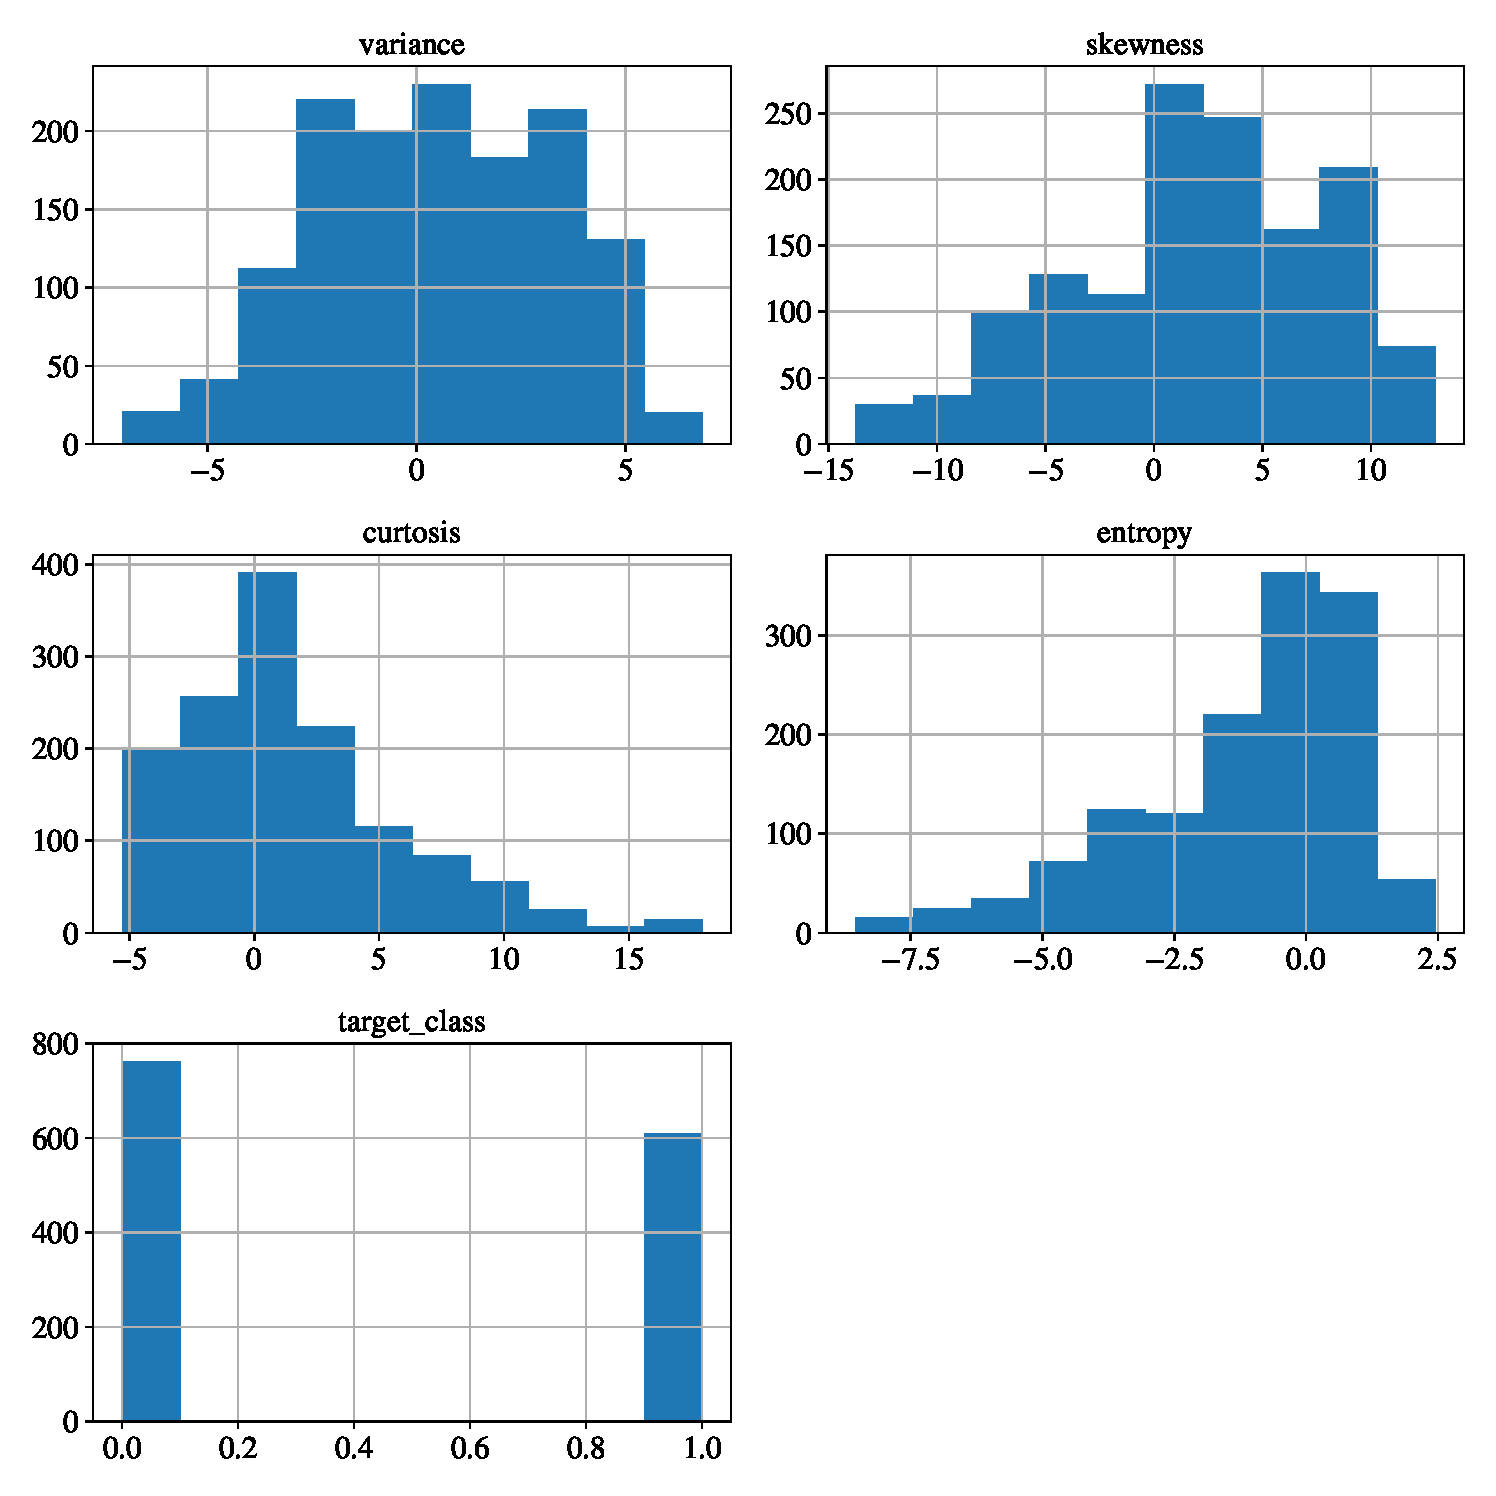
\includegraphics[width=0.7\textwidth]{Histogram.eps}
\caption{Histograms of all four features and the target class.}
\end{figure}
\textbf{Interpretation:} Variance and skewness are more or less spread out evenly, kind of like a normal curve. curtosis and entropy are not like that — they lean more to one side, entropy especially has a lot of values crowded near the negative side. The target class graph shows we have a bit more authentic notes than forged ones, but not by a huge margin.

\subsection*{9.2 Correlation Heatmap}
\begin{figure}[H]
\centering
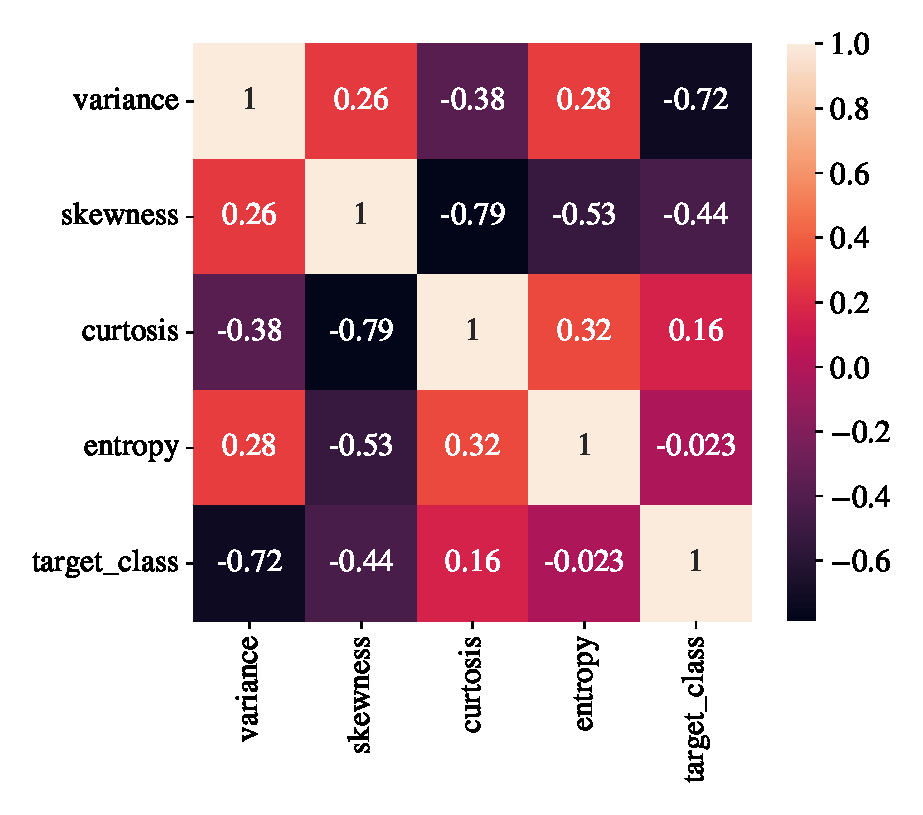
\includegraphics[width=0.55\textwidth]{co-relation-heatmap.eps}
\caption{Correlation heatmap of all features.}
\end{figure}
\textbf{Interpretation:} Variance has the strongest correlation with the target class, around $-0.72$, so this feature alone tells us a lot about whether a note is real or fake. Skewness and curtosis are strongly negatively correlated with each other (around $-0.79$), meaning when one goes up the other usually goes down. None of the features are copies of each other, so all four are useful to keep.

\subsection*{9.3 Scatter Plot}
\begin{figure}[H]
\centering
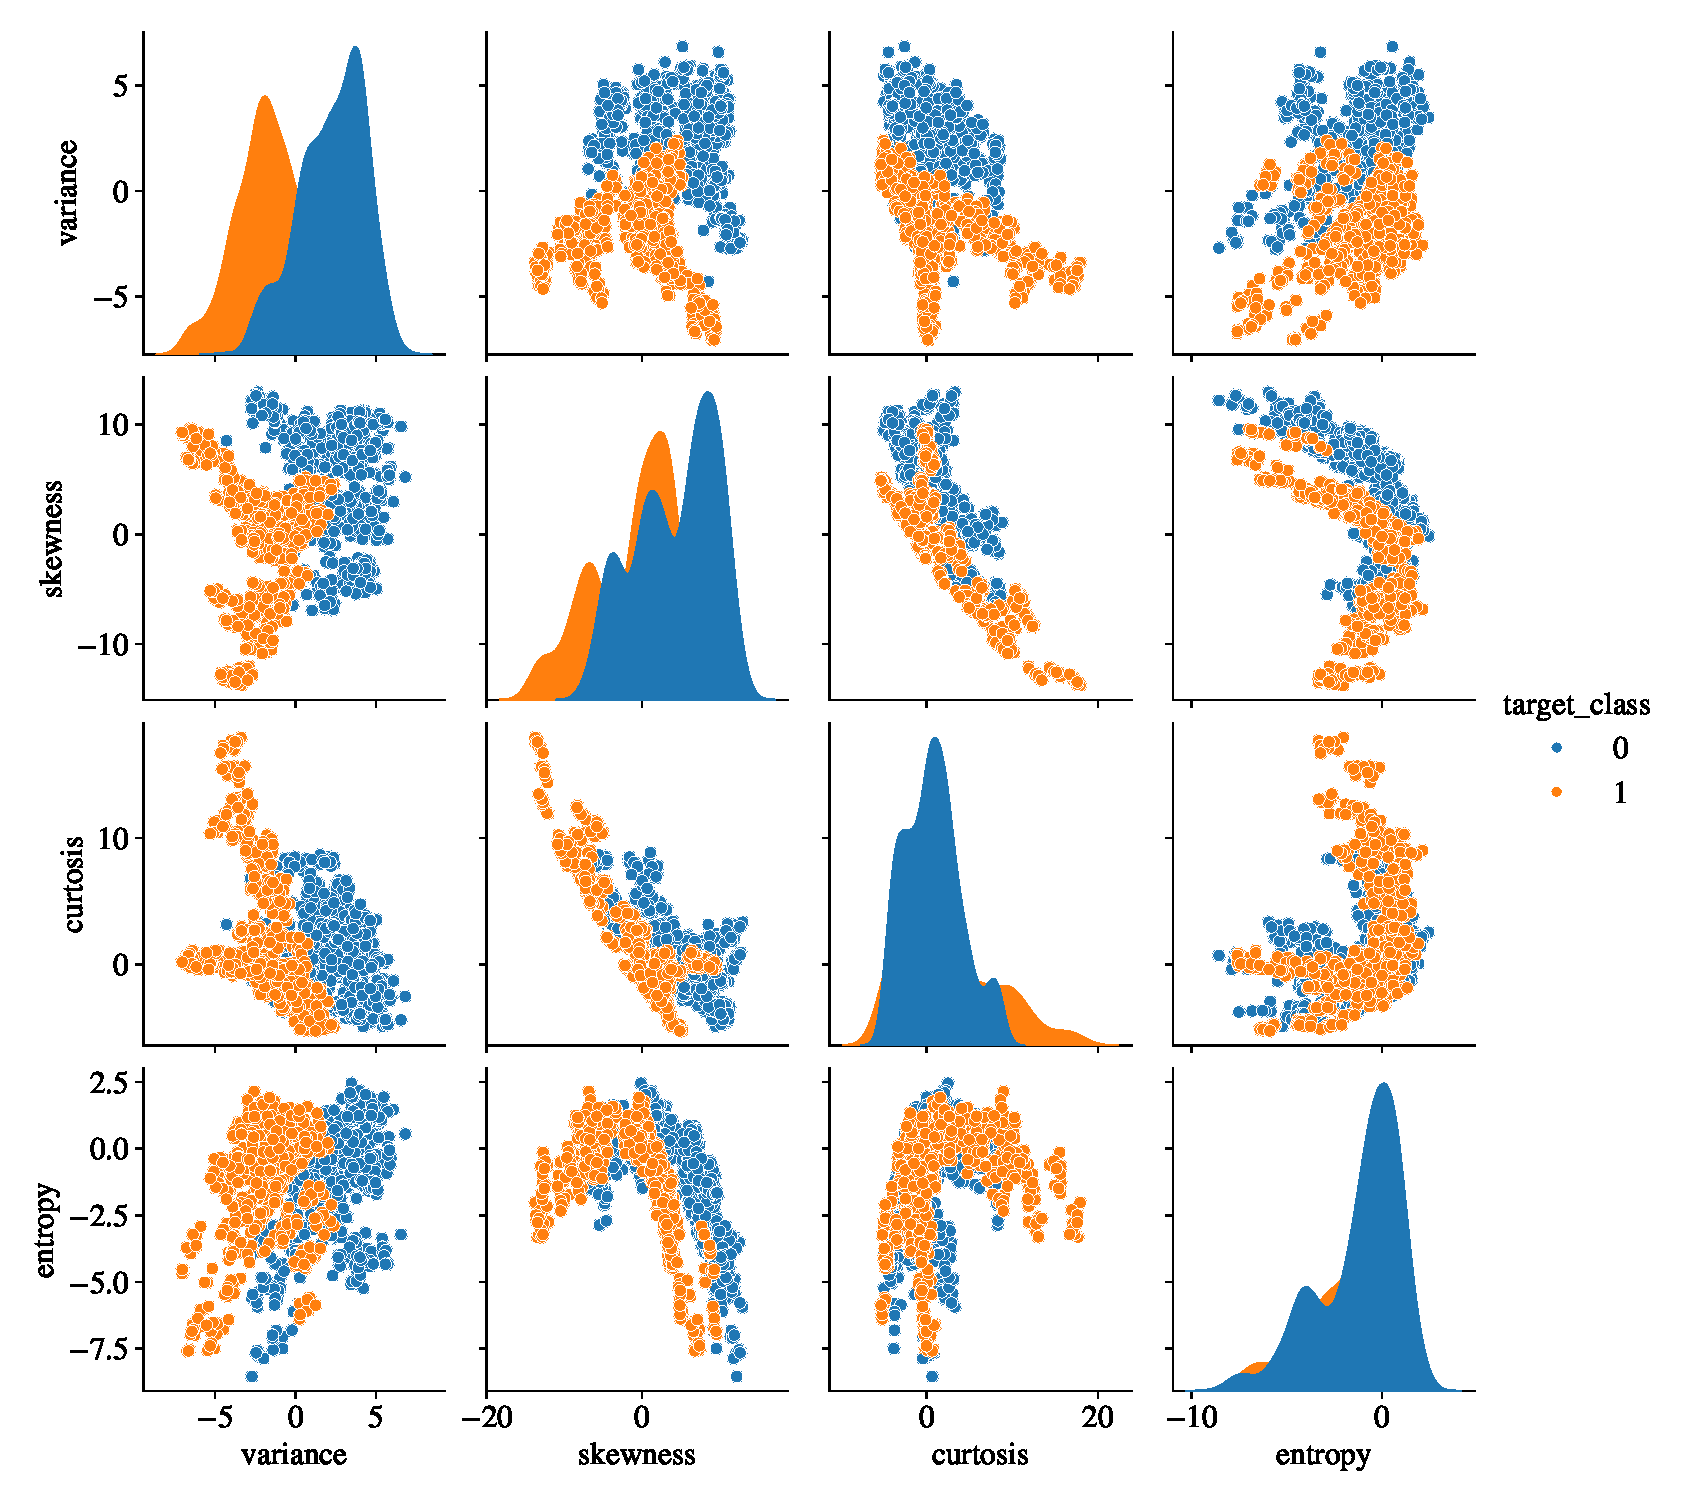
\includegraphics[width=0.8\textwidth]{scatterplot.eps}
\caption{Pairwise scatter plot coloured by class.}
\end{figure}
\textbf{Interpretation:} When we look at variance and skewness together, the blue points (authentic) and orange points (forged) form two separate groups, with only a little overlap in the middle. This tells us the classes are almost linearly separable, which is a good sign for a perceptron since it can only draw straight line boundaries. This overlap is also probably why our model didn't get 100\% accuracy.

\subsection*{9.4 Box Plots}
\begin{figure}[H]
\centering
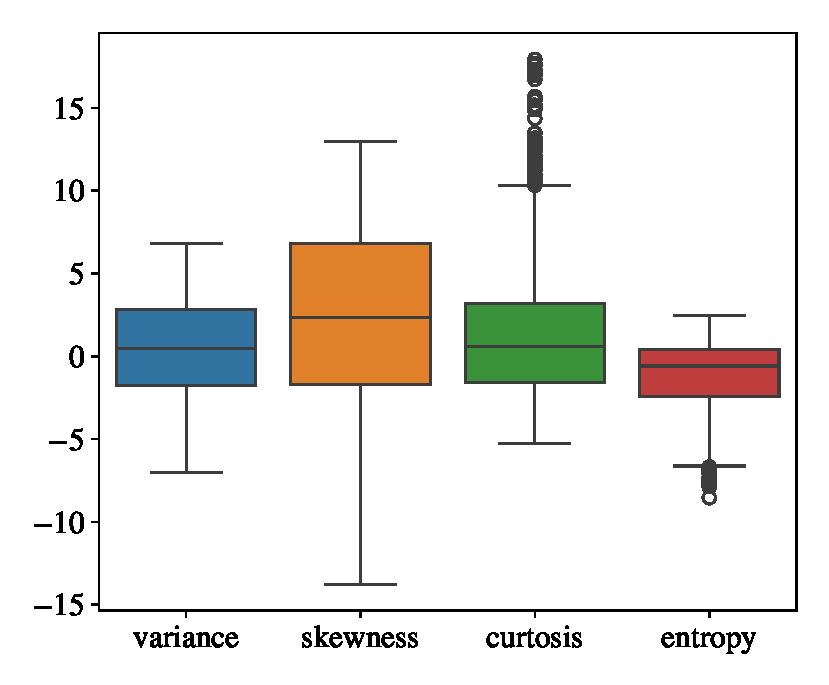
\includegraphics[width=0.6\textwidth]{box-plot.eps}
\caption{Box plots of the four features.}
\end{figure}
\textbf{Interpretation:} Skewness has the widest range and biggest spread out of all the features. curtosis has quite a few outlier points sitting above the upper whisker. Since the features have very different ranges before scaling, this is exactly why we needed to normalize everything before training the perceptron.

\subsection*{9.5 Training Error vs Epoch}
\begin{figure}[H]
\centering
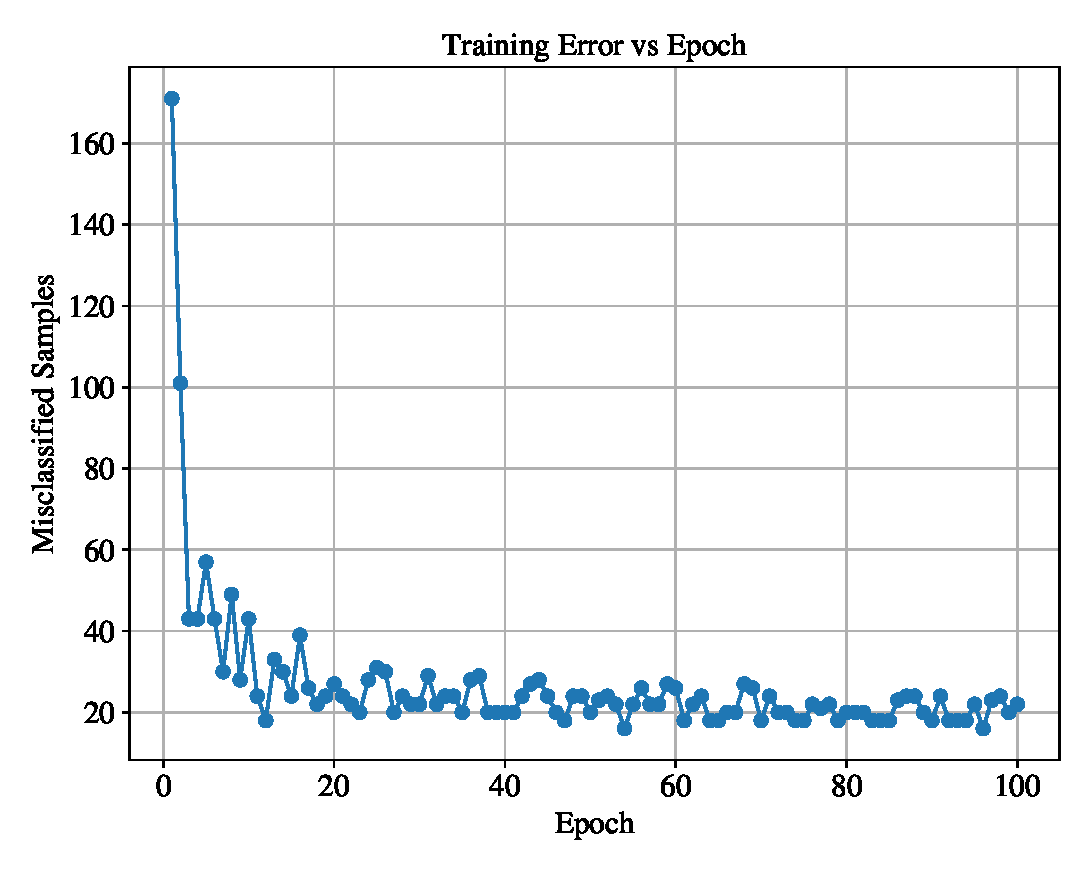
\includegraphics[width=0.65\textwidth]{training-error-vs-epoch.eps}
\caption{Misclassified samples per epoch, learning rate = 0.01.}
\end{figure}
\textbf{Interpretation:} The error drops really fast in the first 10 epochs, from 171 wrong predictions down to under 30. After that point, it doesn't go to zero — it just keeps bouncing between about 16 and 30 errors till epoch 100. This happens because a few points from both classes overlap each other, so the perceptron keeps correcting the same handful of points again and again without ever fully settling down.

\subsection*{9.6 Weight Evolution}
\begin{figure}[H]
\centering
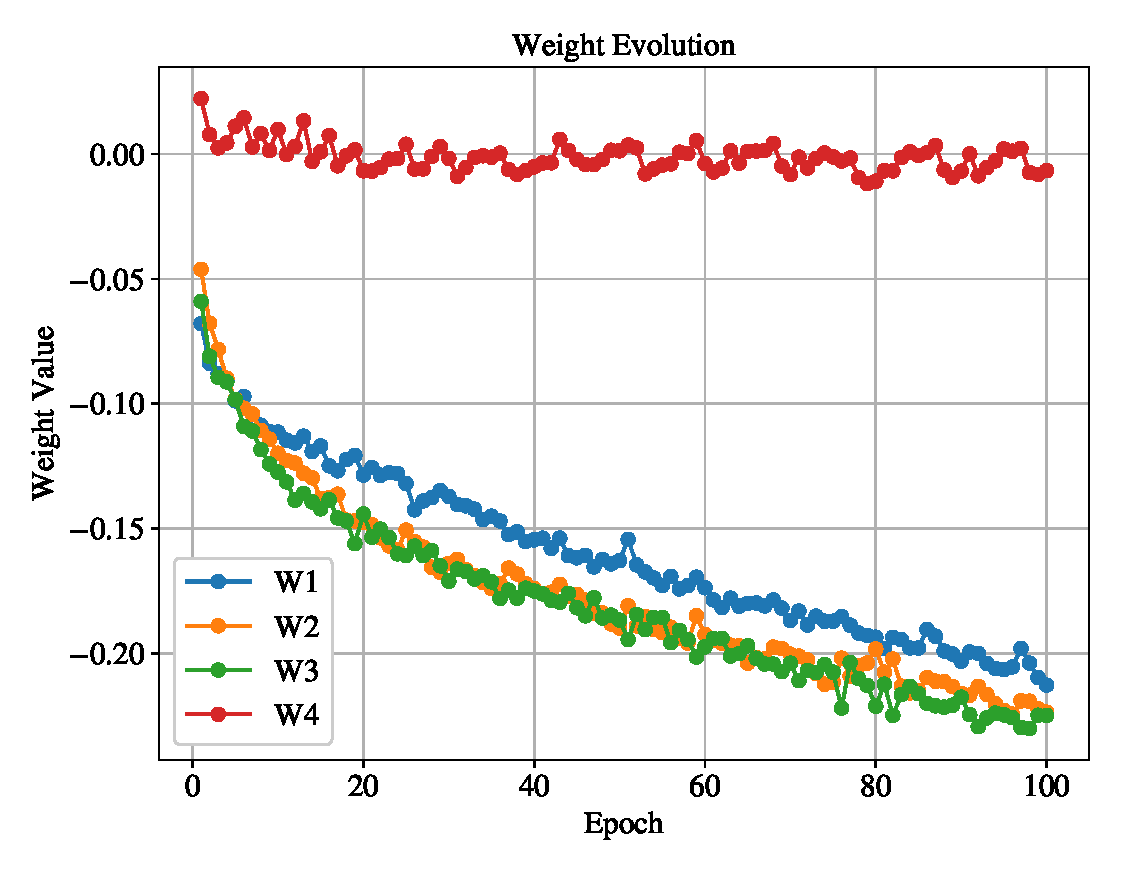
\includegraphics[width=0.65\textwidth]{weight-evolution.eps}
\caption{Weight values over 100 epochs.}
\end{figure}
\textbf{Interpretation:} All four weights start at 0 (as we set them) and move down into negative values pretty quickly within the first 15 epochs. After that, they mostly flatten out and just move a little here and there instead of changing a lot. This basically means the model found its rough decision boundary early on and spent the rest of the epochs just adjusting it slightly.

\subsection*{9.7 Bias Evolution}
\begin{figure}[H]
\centering
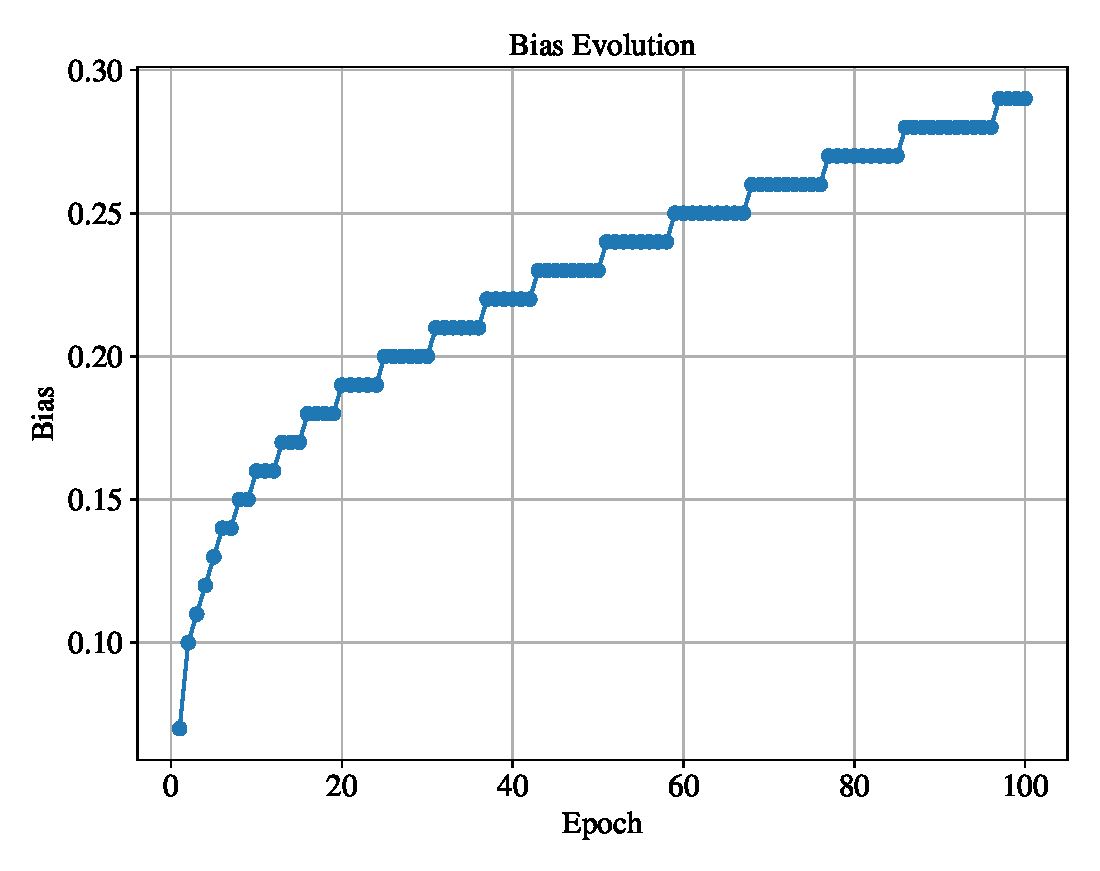
\includegraphics[width=0.65\textwidth]{bias-evolution.eps}
\caption{Bias value over 100 epochs.}
\end{figure}
\textbf{Interpretation:} Unlike the weights, the bias keeps climbing up slowly and steadily throughout training, going from 0 to almost 0.29 by the end, like a staircase. It never really flattens out completely because misclassifications keep happening every epoch, even if the count is small, and each one nudges the bias up a tiny bit more.

\subsection*{9.8 Confusion Matrix}
\begin{figure}[H]
\centering
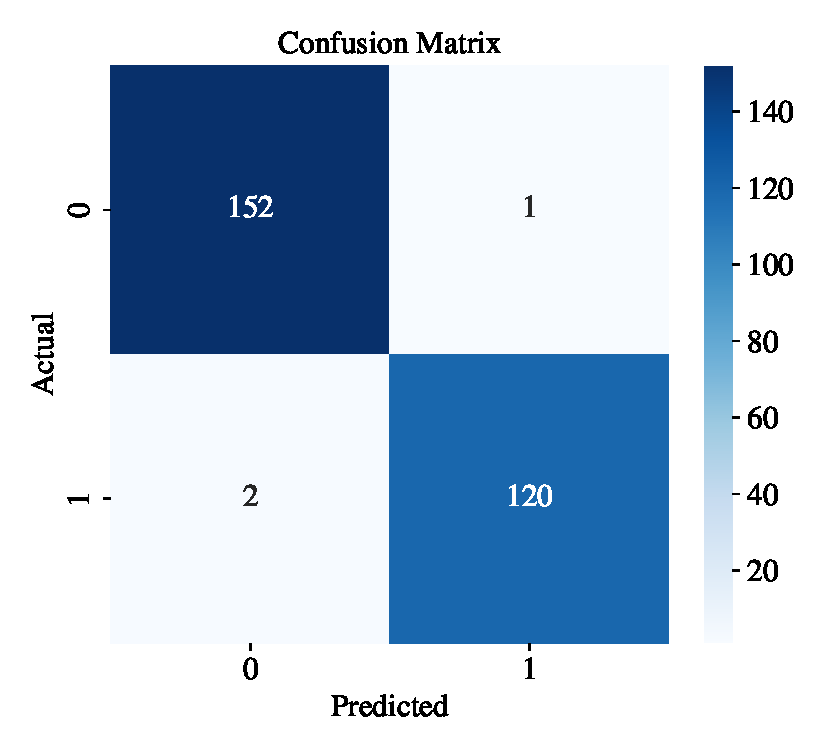
\includegraphics[width=0.5\textwidth]{confusion-matrix.eps}
\caption{Confusion matrix on test data.}
\end{figure}
\textbf{Interpretation:} Out of 275 test samples, our model got 152 authentic notes and 120 forged notes correct, and only messed up 3 samples total (1 false positive, 2 false negatives). This means the model works really well on data it has never seen before, not just on the training data.

\subsection*{9.9 Learning Rate Comparison}
\begin{figure}[H]
\centering
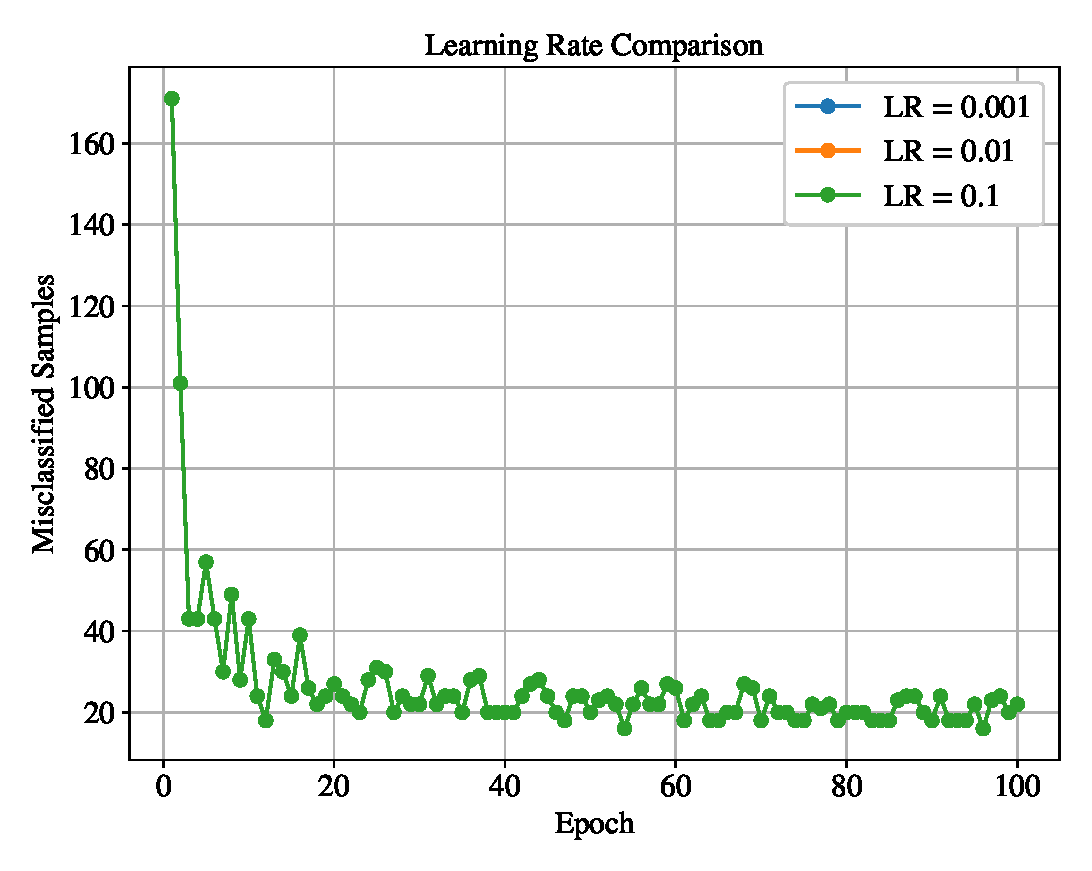
\includegraphics[width=0.65\textwidth]{learning_comparission_rate.eps}
\caption{Error curves for learning rates 0.001, 0.01, 0.1.}
\end{figure}
\textbf{Interpretation:} Looking at the graph carefully, only the green line (LR = 0.1) is visible even though all three learning rates are plotted — this is because all three curves are exactly overlapping each other, not just similar. This happens because our weights start at zero, and the perceptron update rule only scales the weight and bias values by the learning rate — it doesn't change whether a point gets classified correctly or not, since that only depends on the sign of the output, not its size. So changing the learning rate only changes how big the weight numbers get, not the actual predictions made at each epoch. That's exactly why all three learning rates ended up with the identical error curve and the identical final test accuracy of 98.91 percent.
%----------------------------------------------------------

\section*{10. Performance Tables}

\textbf{Training Summary}

\begin{table}[h]
\centering
\caption{Model Training Parameters and Performance}
\begin{tabular}{|l|l|}
\hline
\textbf{Parameter} & \textbf{Value} \\ \hline
Dataset Size & 1372 samples \\ \hline
Train/Test Split & 1097 / 275 (80/20, stratified) \\ \hline
Learning Rate & 0.01 \\ \hline
Epochs & 100 (did not fully converge, kept oscillating) \\ \hline
Final Weights & [-0.2126, -0.2234, -0.2247, -0.0067] \\ \hline
Final Bias & 0.29 \\ \hline
Accuracy & 0.9891 \\ \hline
Precision & 0.9917 \\ \hline
Recall & 0.9836 \\ \hline
F1-score & 0.9877 \\ \hline
\end{tabular}
\label{tab:model_results}
\end{table}

\vspace{3mm}

\textbf{Epoch-wise Learning}

\begin{table}[h]
\centering
\caption{Epoch-wise Learning Progress}
\begin{tabular}{|c|c|c|c|c|}
\hline
\textbf{Epoch} & \textbf{Errors} & \textbf{Weight 1} & \textbf{Weight 2} & \textbf{Bias} \\
\hline
1   & 171 & -0.0679 & -0.0462 & 0.07 \\
25  & 31  & -0.1319 & -0.1506 & 0.20 \\
50  & 20  & -0.1628 & -0.1898 & 0.23 \\
75  & 18  & -0.1871 & -0.2114 & 0.26 \\
100 & 22  & -0.2126 & -0.2234 & 0.29 \\
\hline
\end{tabular}

\label{tab:epoch_learning}
\end{table}

%----------------------------------------------------------

\section*{11. Additional Tasks}

\begin{enumerate}[leftmargin=*]
\item Compare the Step and Sigmoid activation functions. Discuss why the Step Activation Function is not used in modern deep learning models.
\\
\textit{Answer : Step function gives 0 if f(x) < 0 and 1 when f(x)>0, and it has slope 0 everywhere except at 0 hence we cannot use it with gradient descent, Sigmoid on the other hand gives values between 0 and 1 and has smooth slopes everywhere, so it works with backpropagation, thats why modern deep learning models use sigmoid and not step.}
\item Compare the implementation with Scikit-learn's Perceptron.
\\
\textit{Answer : Both the ideas are same , which is updating the weights, but the scikit version is more optimized but our version lets us see the error, weight and bias values epoch by epoch.}
\item Repeat the experiment using learning rates 0.001, 0.01 and 0.1.
\\
\textit{Answer :All three learning rates (0.001, 0.01, 0.1) produced the exact same error curve and the same final test accuracy of 98.91. This is because the perceptron was initialized with zero weights, and the learning rate only scales the size of the weight updates it doesn't affect the sign of the prediction, which is what decides right or wrong. So the three models made identical classification decisions at every epoch, just with different-sized weight numbers underneath. This would not stay true if the weights were initialized to non-zero random values instead of zero. .}
\item Explain why a Single Layer Perceptron cannot solve the XOR problem.
\\
\textit{Answer : In XOR, the points (0,1) and (1,0) give output 1, and (0,0) and (1,1) give output 0s since these points are placed diagonally opposite, it is not possible for a straight line to seperate them, but a perceptron can only draw a straight boundry, hence a single layer perceptron cannot solve XOR problem and we need multiple layers.}
\item Study the effect of feature normalization on model convergence.
\\
\textit{Answer : Before normalizing, features like entropy (range -8.5 to 2.4) and skewness (range -14 to 13) were on totally different scales, which would mess up the weight updates unfairly. After Min-Max scaling everything to 0-1, all features got treated equally, and that's a big reason the model reached a low-error zone within just 10-15 epochs..}
\end{enumerate}

%----------------------------------------------------------
\section*{12. Discussion}

The perceptron worked really well on this dataset, getting about 98.9\% accuracy on data it never saw during training. But it's worth pointing out that it never actually reached 0 errors during training — the error count kept jumping between 16 and 30 samples out of 1097, even after 100 epochs. This is because the two classes overlap a little bit (seen clearly in the scatter plot), so the data is not perfectly linearly separable, just close to it. The learning rate comparison also showed something interesting — even though the three rates behaved very differently while training, all of them landed on the same final test performance, meaning the learning rate mostly affects the training journey, not the final destination, at least for this dataset.

\section*{13. Conclusion}

We successfully built a Single Layer Perceptron from scratch, without using any built-in ML classifier, and used it to tell apart real and forged banknotes using 4 simple features. After normalizing the data and training for 100 epochs at a learning rate of 0.01, the model reached 98.91\% accuracy, 99.17\% precision, 98.36\% recall and an F1-score of 98.77\% on the test set. The model didn't fully converge because the two classes overlap slightly, but the results are still very strong for a plain single-layer model. This experiment gave a clear, hands-on understanding of how something as basic as the perceptron learning rule can still solve real classification problems fairly accurately.
\section*{12. Report Contents}

The report should include:

\begin{itemize}
\item Objective
\item Background Theory
\item Activation Functions
\item Dataset Description
\item Experimental Procedure
\item Source Code
\item Experimental Results
\item Generated Plots with Interpretation
\item Performance Tables
\item Discussion
\item Conclusion
\item References
\end{itemize}

%----------------------------------------------------------

\section*{14. References}

\begin{enumerate}
\item F. Rosenblatt, ``The Perceptron,'' \emph{Psychological Review}, 1958.
\item I. Goodfellow, Y. Bengio and A. Courville, \emph{Deep Learning}, MIT Press, 2016.
\item C. M. Bishop, \emph{Pattern Recognition and Machine Learning}, Springer, 2006.
\item S. Haykin, \emph{Neural Networks and Learning Machines}, Pearson, 2009.
\item UCI Machine Learning Repository -- Banknote Authentication Dataset.
\item Scikit-learn Documentation: Perceptron.
\end{enumerate}
\vspace{300mm}
\section*{Additional Exercise}
\section{Objective:}
Code the perceptron learning algorithm for OR, NOT, and AND gates using Python. Show the weights after each update. Plot the decision boundary after each weight update using Python built-in packages. (K4)

\section{Methodology}

A single-layer perceptron was implemented from scratch for each logic gate. The weights and bias were initialized to zero, and the step activation function was used to generate binary outputs. During each iteration, the prediction error was computed and the weights and bias were updated using the Perceptron Learning Rule. The training process continued until all input patterns were classified correctly. The evolution of the decision boundary was visualized after every parameter update.

\section{Experimental Procedure}

The truth tables corresponding to the AND, OR, NAND, NOR, and NOT logic gates were used as the training dataset. The perceptron was trained with a learning rate of 1 and zero initialization for both weights and bias. During training, the weight and bias values were updated whenever a misclassification occurred. The learning process terminated when all training samples were classified correctly. The source code used for implementing the perceptron is available in the GitHub repository.

\ Source Code :
\url{https://github.com/Siddharth-G06/Deep-Learning-Lab/tree/main/Lab%201%20-%20Single%20Layer%20Perceptron}

\section{Results}

The perceptron successfully learned all linearly separable logic gates. The final weight and bias values correctly classified all training samples. The decision boundary plots generated after each update illustrate the gradual adjustment of the separating hyperplane until convergence.

\begin{figure}[H]
    \centering
    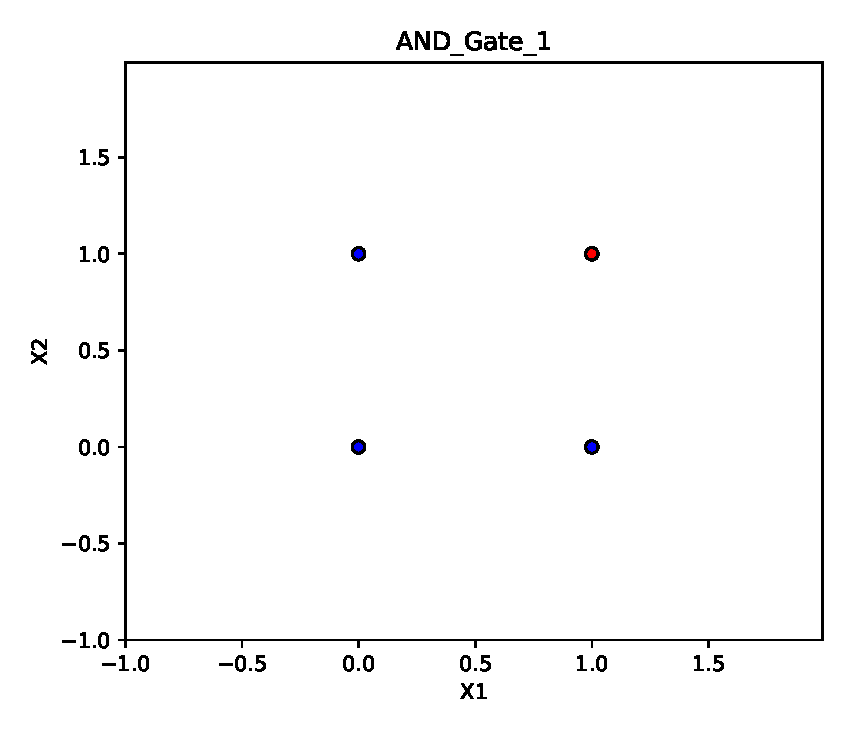
\includegraphics[width=0.55\textwidth]{AND_Gate_1.eps}
    \caption{Decision boundary after Epoch 1 for the AND gate.}
\end{figure}

\begin{figure}[H]
    \centering
    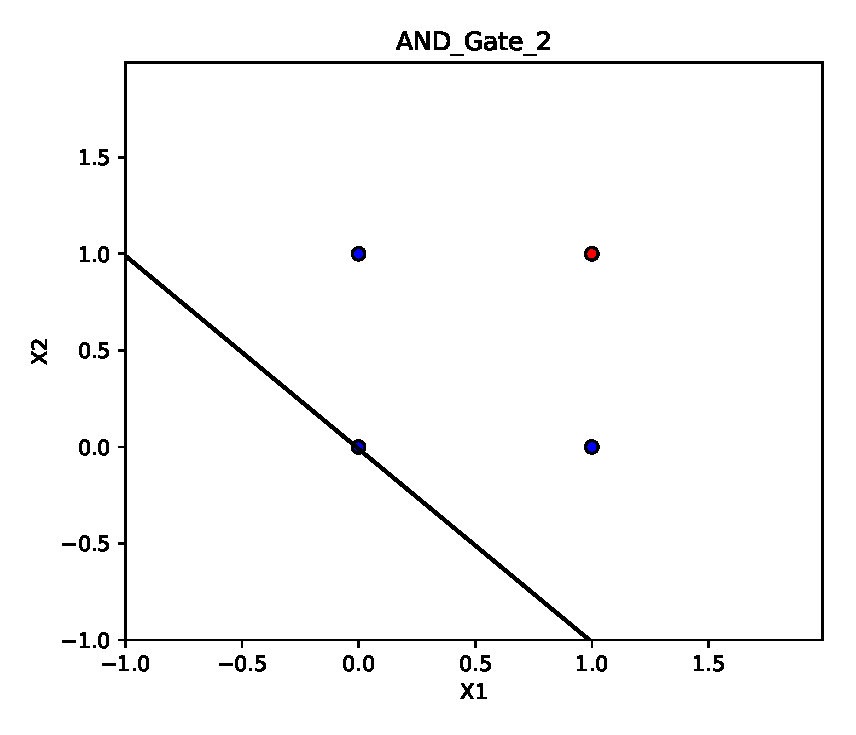
\includegraphics[width=0.55\textwidth]{AND_Gate_2.eps}
    \caption{Decision boundary after Epoch 2 for the AND gate.}
\end{figure}

\begin{figure}[H]
    \centering
    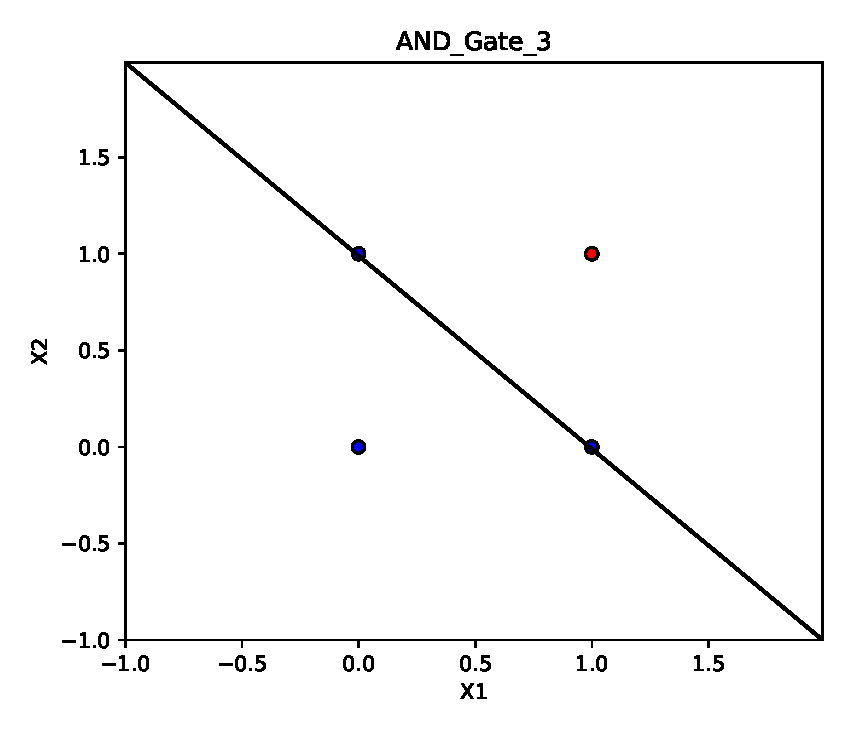
\includegraphics[width=0.55\textwidth]{AND_Gate_3.eps}
    \caption{Decision boundary after Epoch 3 for the AND gate.}
\end{figure}

\begin{figure}[H]
    \centering
    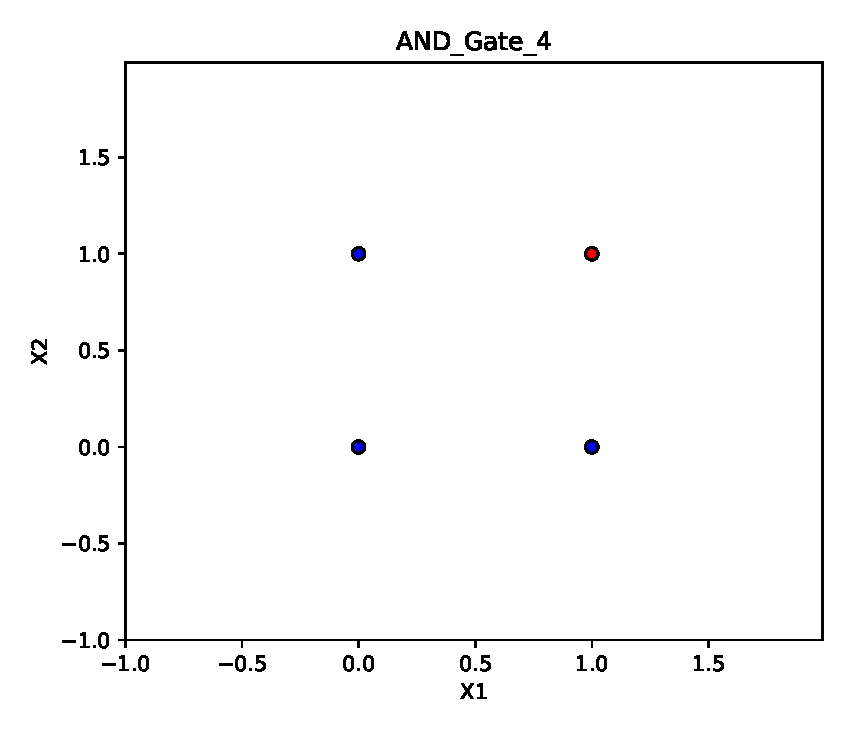
\includegraphics[width=0.55\textwidth]{AND_Gate_4.eps}
    \caption{Decision boundary after Epoch 4 for the AND gate.}
\end{figure}

\begin{figure}[H]
    \centering
    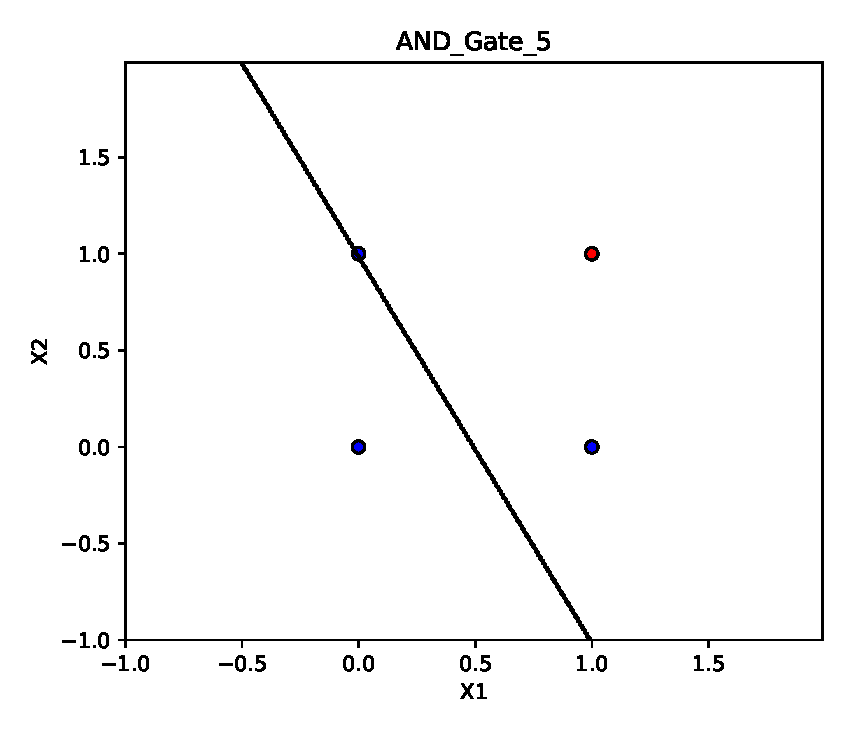
\includegraphics[width=0.55\textwidth]{AND_Gate_5.eps}
    \caption{Decision boundary after Epoch 5 for the AND gate.}
\end{figure}

\begin{figure}[H]
    \centering
    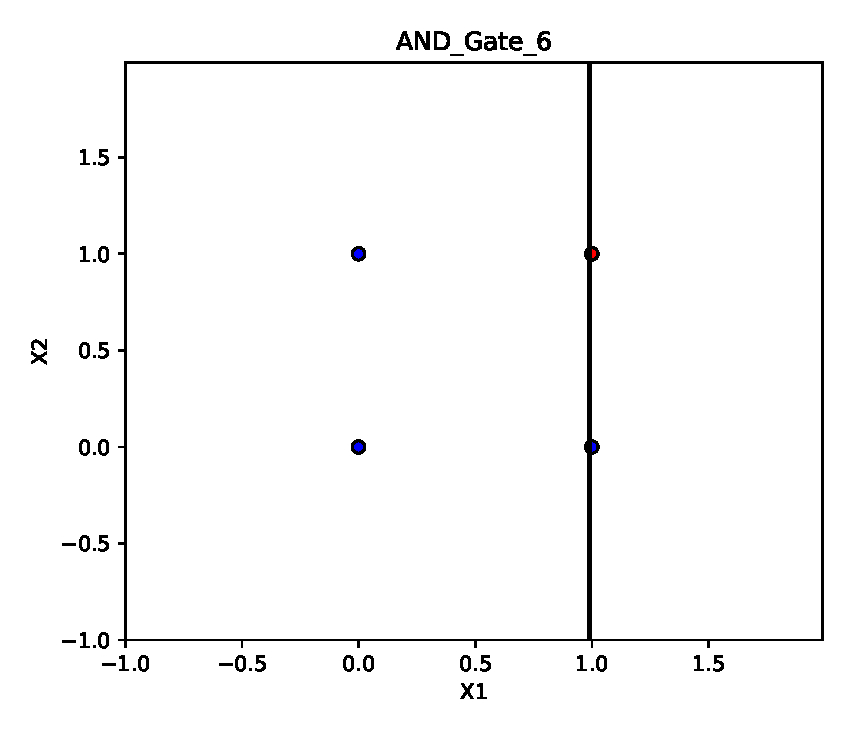
\includegraphics[width=0.55\textwidth]{AND_Gate_6.eps}
    \caption{Decision boundary after Epoch 6 for the AND gate.}
\end{figure}

\begin{figure}[H]
    \centering
    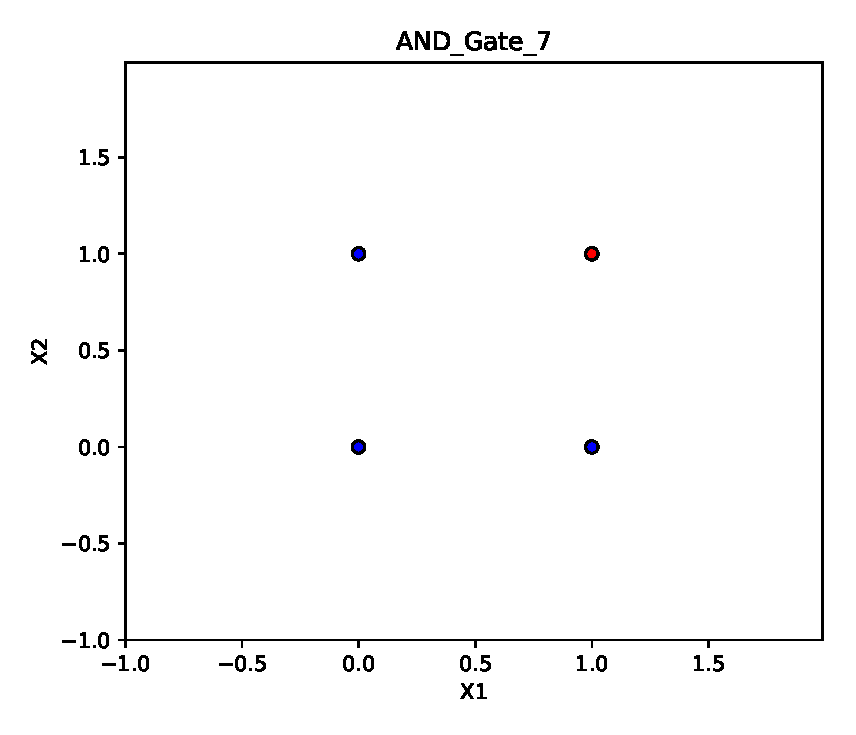
\includegraphics[width=0.55\textwidth]{AND_Gate_7.eps}
    \caption{Decision boundary after Epoch 7 for the AND gate.}
\end{figure}

\begin{figure}[H]
    \centering
    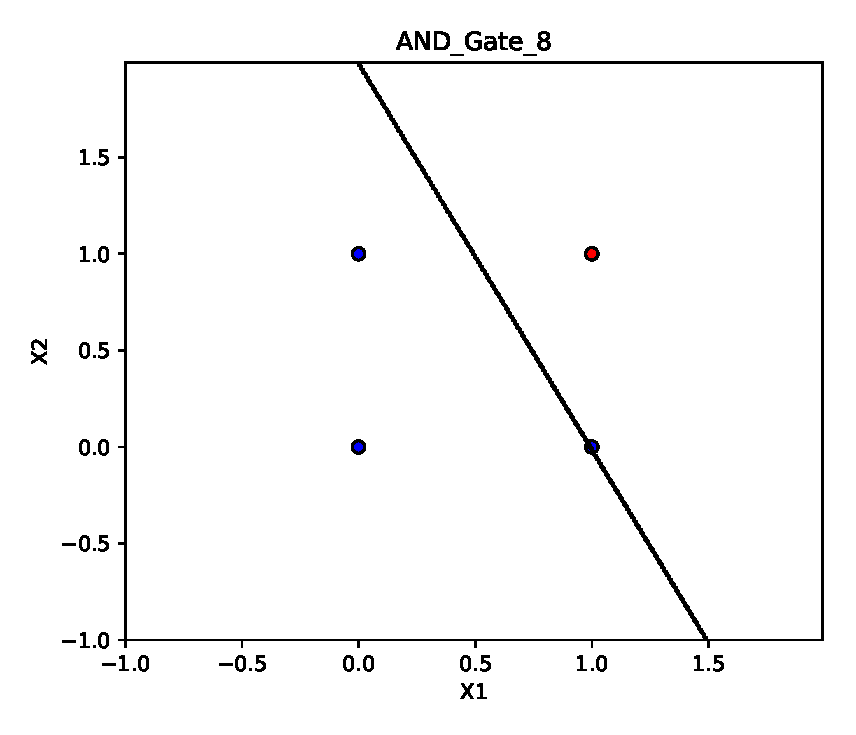
\includegraphics[width=0.55\textwidth]{AND_Gate_8.eps}
    \caption{Decision boundary after Epoch 8 for the AND gate.}
\end{figure}

\begin{figure}[H]
    \centering
    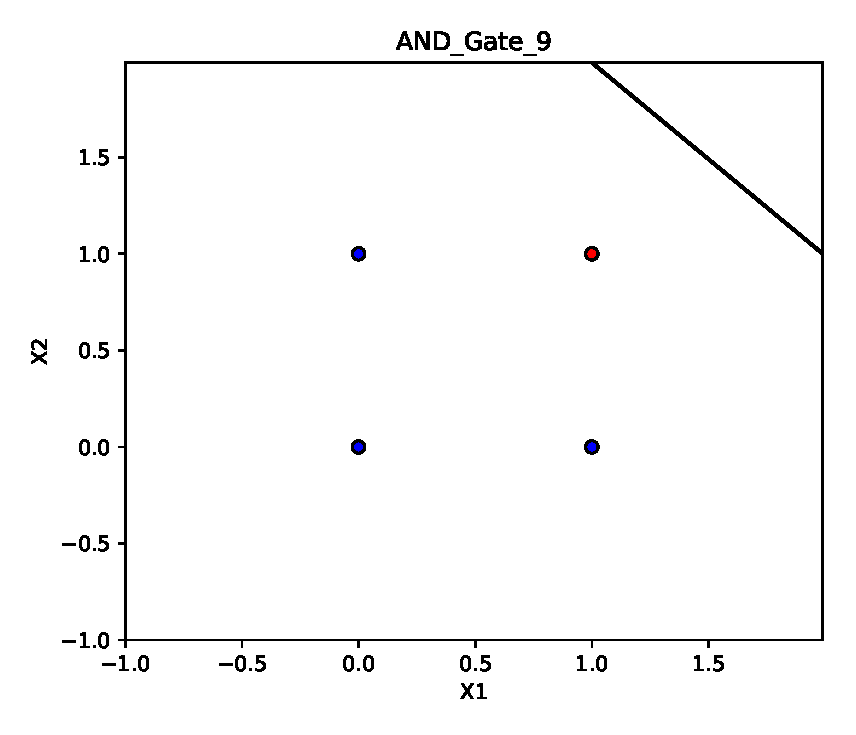
\includegraphics[width=0.55\textwidth]{AND_Gate_9.eps}
    \caption{Decision boundary after Epoch 9 for the AND gate.}
\end{figure}

\begin{figure}[H]
    \centering
    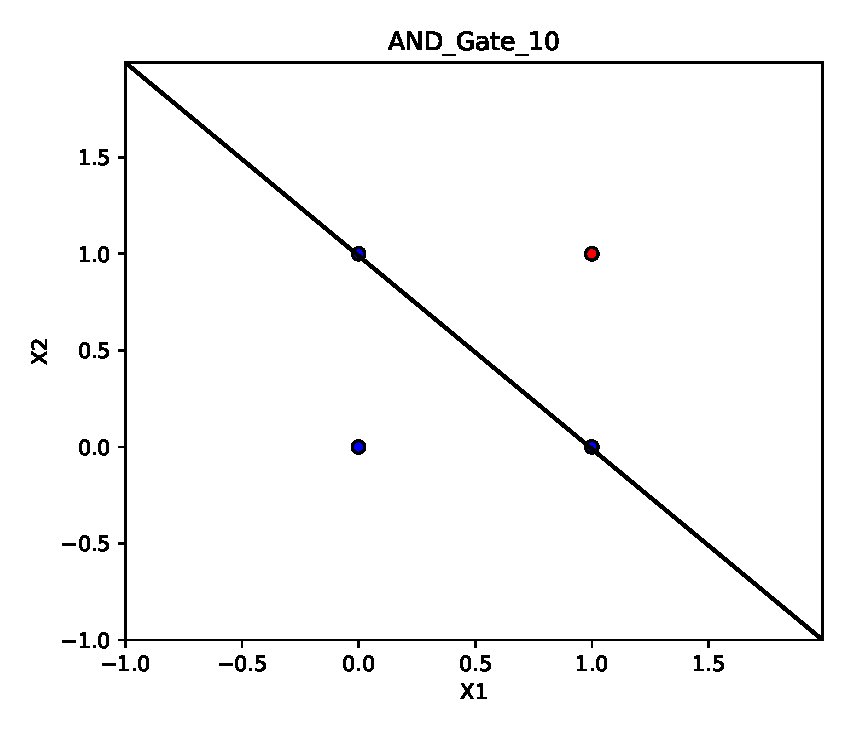
\includegraphics[width=0.55\textwidth]{AND_Gate_10.eps}
    \caption{Decision boundary after Epoch 10 for the AND gate.}
\end{figure}

\begin{figure}[H]
    \centering
    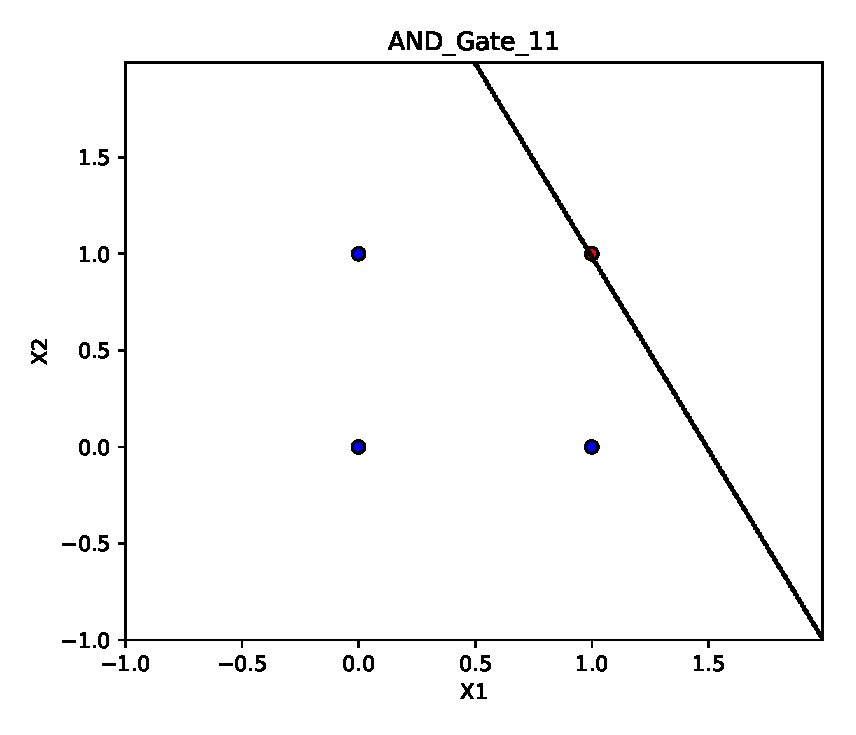
\includegraphics[width=0.55\textwidth]{AND_Gate_11.eps}
    \caption{Decision boundary after Epoch 11 for the AND gate.}
\end{figure}

\begin{figure}[H]
    \centering
    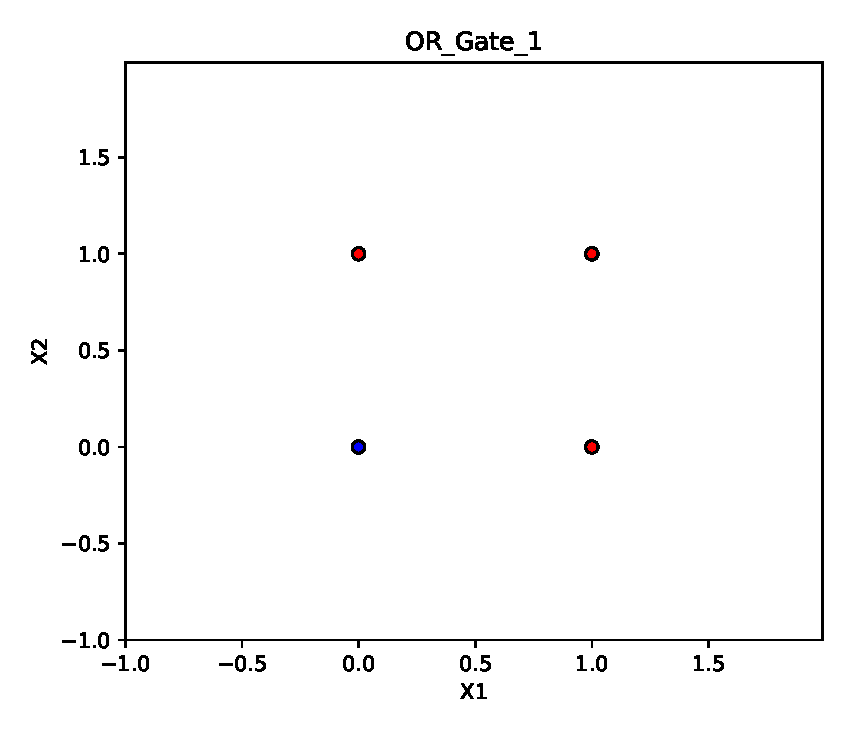
\includegraphics[width=0.55\textwidth]{OR_Gate_1.eps}
    \caption{Decision boundary after Epoch 1 for the OR gate.}
\end{figure}

\begin{figure}[H]
    \centering
    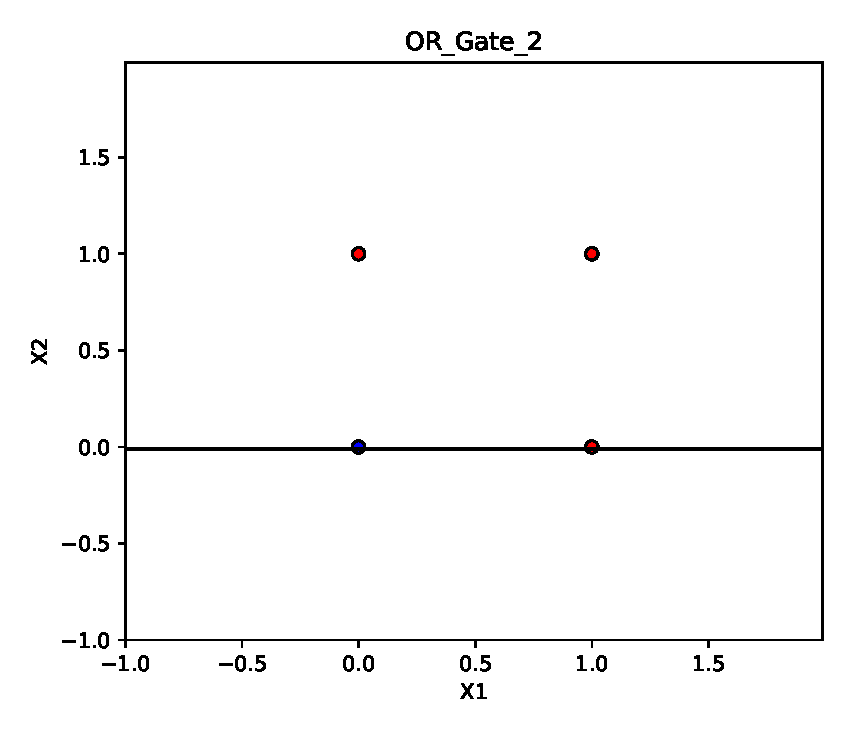
\includegraphics[width=0.55\textwidth]{OR_Gate_2.eps}
    \caption{Decision boundary after Epoch 2 for the OR gate.}
\end{figure}
\begin{figure}[H]
    \centering
    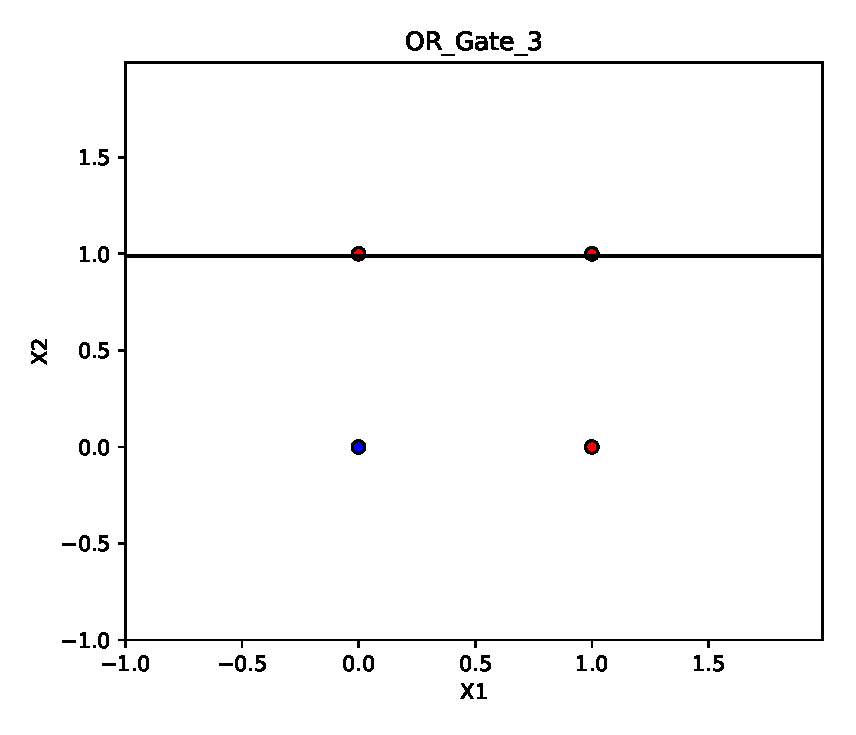
\includegraphics[width=0.55\textwidth]{OR_Gate_3.eps}
    \caption{Decision boundary after Epoch 1 for the OR gate.}
\end{figure}

\begin{figure}[H]
    \centering
    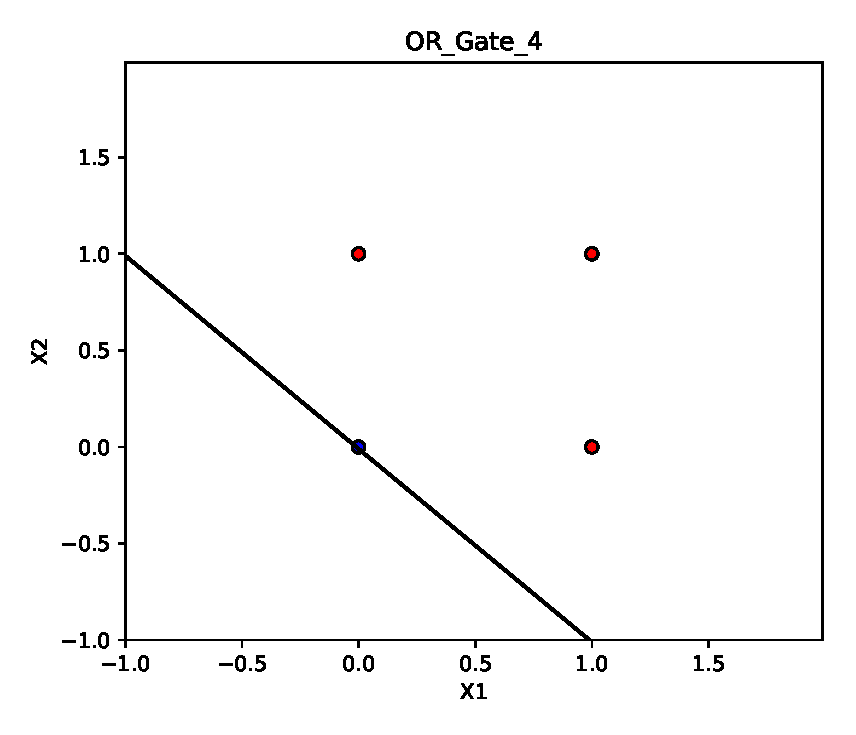
\includegraphics[width=0.55\textwidth]{OR_Gate_4.eps}
    \caption{Decision boundary after Epoch 2 for the OR gate.}
\end{figure}
\begin{figure}[H]
    \centering
    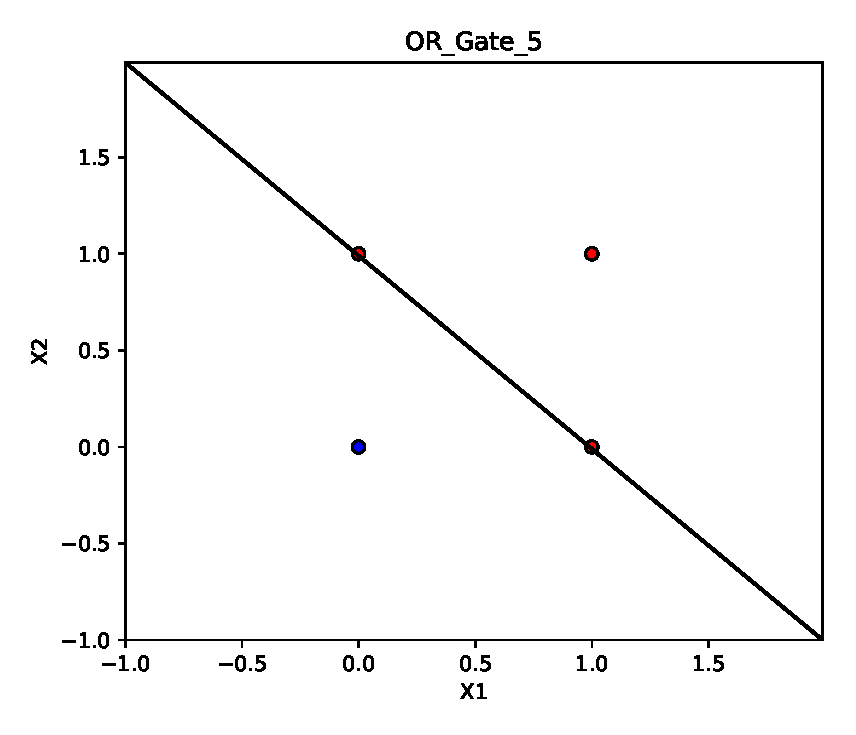
\includegraphics[width=0.55\textwidth]{OR_Gate_5.eps}
    \caption{Decision boundary after Epoch 2 for the OR gate.}
\end{figure}

\begin{figure}[H]
    \centering
    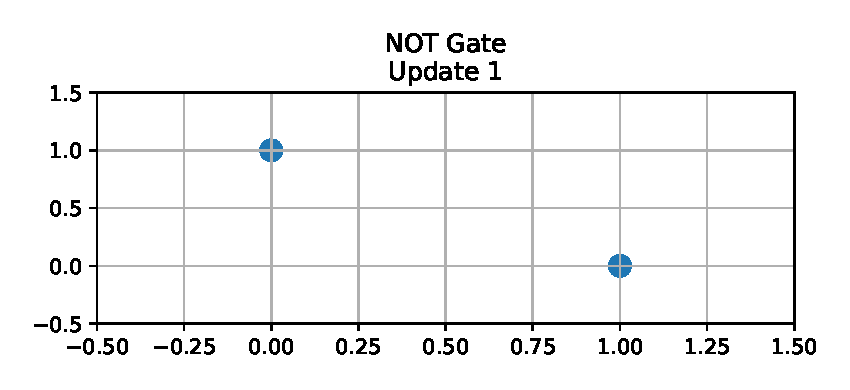
\includegraphics[width=0.55\textwidth]{NOT_Gate_1.eps}
    \caption{Decision boundary after Epoch 1 for the NOT gate.}
\end{figure}

\begin{figure}[H]
    \centering
    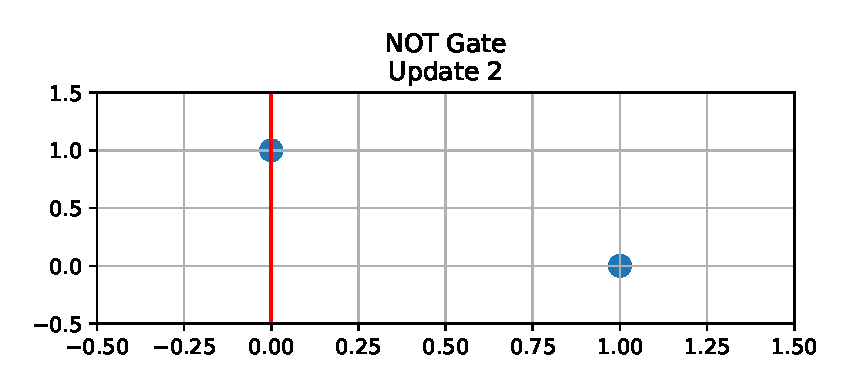
\includegraphics[width=0.55\textwidth]{NOT_Gate_2.eps}
    \caption{Decision boundary after Epoch 2 for the NOT gate.}
\end{figure}

The perceptron successfully learned all linearly separable logic gates. The final weight and bias values correctly classified all training samples. The decision boundary plots generated after each update illustrate the gradual adjustment of the separating hyperplane until convergence.

\section{Conclusion}

The Perceptron Learning Algorithm was successfully implemented for the AND, OR, NAND, NOR, and NOT logic gates. The experiment demonstrated the effectiveness of the perceptron in learning linearly separable problems through iterative updates of the model parameters. The decision boundary visualizations further illustrated the convergence behavior of the algorithm and enhanced the understanding of the perceptron learning process.

\end{document}

